% !BIB TS-program = biber

\RequirePackage[l2tabu,orthodox]{nag}

% TODO: decide if one-sided/two-sided
%\documentclass[headsepline,footsepline,footinclude=false,fontsize=11pt,paper=a4,listof=totoc,bibliography=totoc,BCOR=12mm,DIV=12]{scrbook} % two-sided
\documentclass[headsepline,footsepline,footinclude=false,oneside,fontsize=11pt,paper=a4,listof=totoc,bibliography=totoc]{scrbook} % one-sided

% TODO: change citation style in settings
\PassOptionsToPackage{table,svgnames,dvipsnames}{xcolor}

\usepackage[utf8]{inputenc}
\usepackage[T1]{fontenc}
\usepackage[sc]{mathpazo}
\usepackage[ngerman,american]{babel}
\usepackage[autostyle]{csquotes}
\usepackage[%
  backend=biber,
  url=false,
  style=alphabetic,
  maxnames=4,
  minnames=3,
  maxbibnames=99,
  giveninits,
  uniquename=init]{biblatex} % TODO: adapt citation style
\usepackage{graphicx}
\usepackage{scrhack} % necessary for listings package
\usepackage{listings}
\usepackage{lstautogobble}
\usepackage{tikz}
\usepackage{pgfplots}
\usepackage{pgfplotstable}
\usepackage{booktabs}
\usepackage[final]{microtype}
\usepackage{caption}
\usepackage[printonlyused]{acronym}
\usepackage[hidelinks]{hyperref} % hidelinks removes colored boxes around references and links
\usepackage{parskip}
\AtBeginDocument{%
	\hypersetup{
		pdftitle=\getTitle,
		pdfauthor=\getAuthor,
	}
}
\usepackage{ifthen}

\addto\extrasamerican{
	\def\lstnumberautorefname{Line}
	\def\chapterautorefname{Chapter}
	\def\sectionautorefname{Section}
	\def\subsectionautorefname{Subsection}
	\def\subsubsectionautorefname{Subsubsection}
}

\addto\extrasngerman{
	\def\lstnumberautorefname{Zeile}
}

% Themes
\ifthenelse{\equal{\detokenize{dark}}{\jobname}}{%
  % Dark theme
  \newcommand{\bg}{black} % background
  \newcommand{\fg}{white} % foreground
  \usepackage[pagecolor=\bg]{pagecolor}
  \color{\fg}
}{%
  % Light theme
  \newcommand{\bg}{white} % background
  \newcommand{\fg}{black} % foreground
}

\bibliography{bibliography}

\setkomafont{disposition}{\normalfont\bfseries} % use serif font for headings
\linespread{1.05} % adjust line spread for mathpazo font

% Add table of contents to PDF bookmarks
\BeforeTOCHead[toc]{{\cleardoublepage\pdfbookmark[0]{\contentsname}{toc}}}

% Define TUM corporate design colors
% Taken from http://portal.mytum.de/corporatedesign/index_print/vorlagen/index_farben
\definecolor{TUMBlue}{HTML}{0065BD}
\definecolor{TUMSecondaryBlue}{HTML}{005293}
\definecolor{TUMSecondaryBlue2}{HTML}{003359}
\definecolor{TUMBlack}{HTML}{000000}
\definecolor{TUMWhite}{HTML}{FFFFFF}
\definecolor{TUMDarkGray}{HTML}{333333}
\definecolor{TUMGray}{HTML}{808080}
\definecolor{TUMLightGray}{HTML}{CCCCC6}
\definecolor{TUMAccentGray}{HTML}{DAD7CB}
\definecolor{TUMAccentOrange}{HTML}{E37222}
\definecolor{TUMAccentGreen}{HTML}{A2AD00}
\definecolor{TUMAccentLightBlue}{HTML}{98C6EA}
\definecolor{TUMAccentBlue}{HTML}{64A0C8}

% Settings for pgfplots
\pgfplotsset{compat=newest}
\pgfplotsset{
  % For available color names, see http://www.latextemplates.com/svgnames-colors
  cycle list={TUMBlue\\TUMAccentOrange\\TUMAccentGreen\\TUMSecondaryBlue2\\TUMDarkGray\\},
}

% Settings for lstlistings
\lstset{%
  basicstyle=\ttfamily,
  columns=fullflexible,
  autogobble,
  keywordstyle=\bfseries\color{TUMBlue},
  stringstyle=\color{TUMAccentGreen},
  captionpos=b
}


% TODO: change thesis information
\newcommand*{\getUniversity}{Technische Universität München}
\newcommand*{\getFaculty}{Informatics}
\newcommand*{\getDegree}{Information Systems}
\newcommand*{\getSchool}{Computation, Information and Technology}
\newcommand*{\getTitle}{Visualization and statistical analysis of performance measurements of database systems}
\newcommand*{\getTitleGer}{Visualisierung und statistische Aufbereitung von Performance Messungen von Datenbanksystemen}
\newcommand*{\getAuthor}{Julian Macias De La Rosa}
\newcommand*{\getDoctype}{Master's Thesis}
\newcommand*{\getSupervisor}{Prof. Thomas Neumann}
\newcommand*{\getAdvisor}{Maximilian Bandle}
\newcommand*{\getSubmissionDate}{20.10.2023}
\newcommand*{\getSubmissionLocation}{Munich}

\usepackage{graphicx}

\begin{document}

% Set page numbering to avoid "destination with the same identifier has been already used" warning for cover page.
% (see https://en.wikibooks.org/wiki/LaTeX/Hyperlinks#Problems_with_Links_and_Pages).
\pagenumbering{alph}
\begin{titlepage}
  % HACK for two-sided documents: ignore binding correction for cover page.
  % Adapted from Markus Kohm's KOMA-Script titlepage=firstiscover handling.
  % See http://mirrors.ctan.org/macros/latex/contrib/koma-script/scrkernel-title.dtx,
  % \maketitle macro.
  \oddsidemargin=\evensidemargin\relax
  \textwidth=\dimexpr\paperwidth-2\evensidemargin-2in\relax
  \hsize=\textwidth\relax

  \centering

  \IfFileExists{logos/tum-logo.pdf}{%
    \includegraphics[height=20mm]{logos/tum-logo.pdf}
  }{%
    \vspace*{20mm}
  }

  \vspace{5mm}
  {\huge\MakeUppercase{School of \getSchool{} --- \getFaculty{}} \par}

  \vspace{5mm}
  {\large\MakeUppercase{\getUniversity{}} \par}

  \vspace{15mm}
  {\Large \getDoctype{} in \getDegree{} \par}

  \vspace{10mm}
  {\huge\bfseries \getTitle{} \par}

  \vspace{10mm}
  {\LARGE \getAuthor{}}

  \IfFileExists{logos/faculty-\fg.pdf}{%
    \vfill{}
    \includegraphics[height=20mm]{logos/faculty-\fg.pdf}
  }{}
\end{titlepage}


\frontmatter{}

\input{pages/title}
\input{pages/disclaimer}
\addcontentsline{toc}{chapter}{Acknowledgments}
\thispagestyle{empty}

\vspace*{20mm}

\begin{center}
    {\usekomafont{sectioning}\usekomafont{section} Acknowledgments}
\end{center}

\vspace{10mm}

I extend my sincere gratitude to my advisor Maximilian Bandle for his invaluable guidance and unwavering support throughout this research journey. His prompt responses and willingness to assist at any time significantly enriched the quality of this work.

I would also like to express my appreciation to Tom Papke for his generous assistance during the integration process of the Query Plan Visualizer. His expertise and collaborative spirit played a crucial role in enhancing the functionality of the Benchy Viewer.

This research would not have been possible without the encouragement and support of these individuals, and I am truly thankful for their contributions to the successful completion of this thesis.

\cleardoublepage{}

\chapter{\abstractname}

\begin{figure}[h]
    \centering
    \begin{subfigure}[b]{0.3\linewidth}
      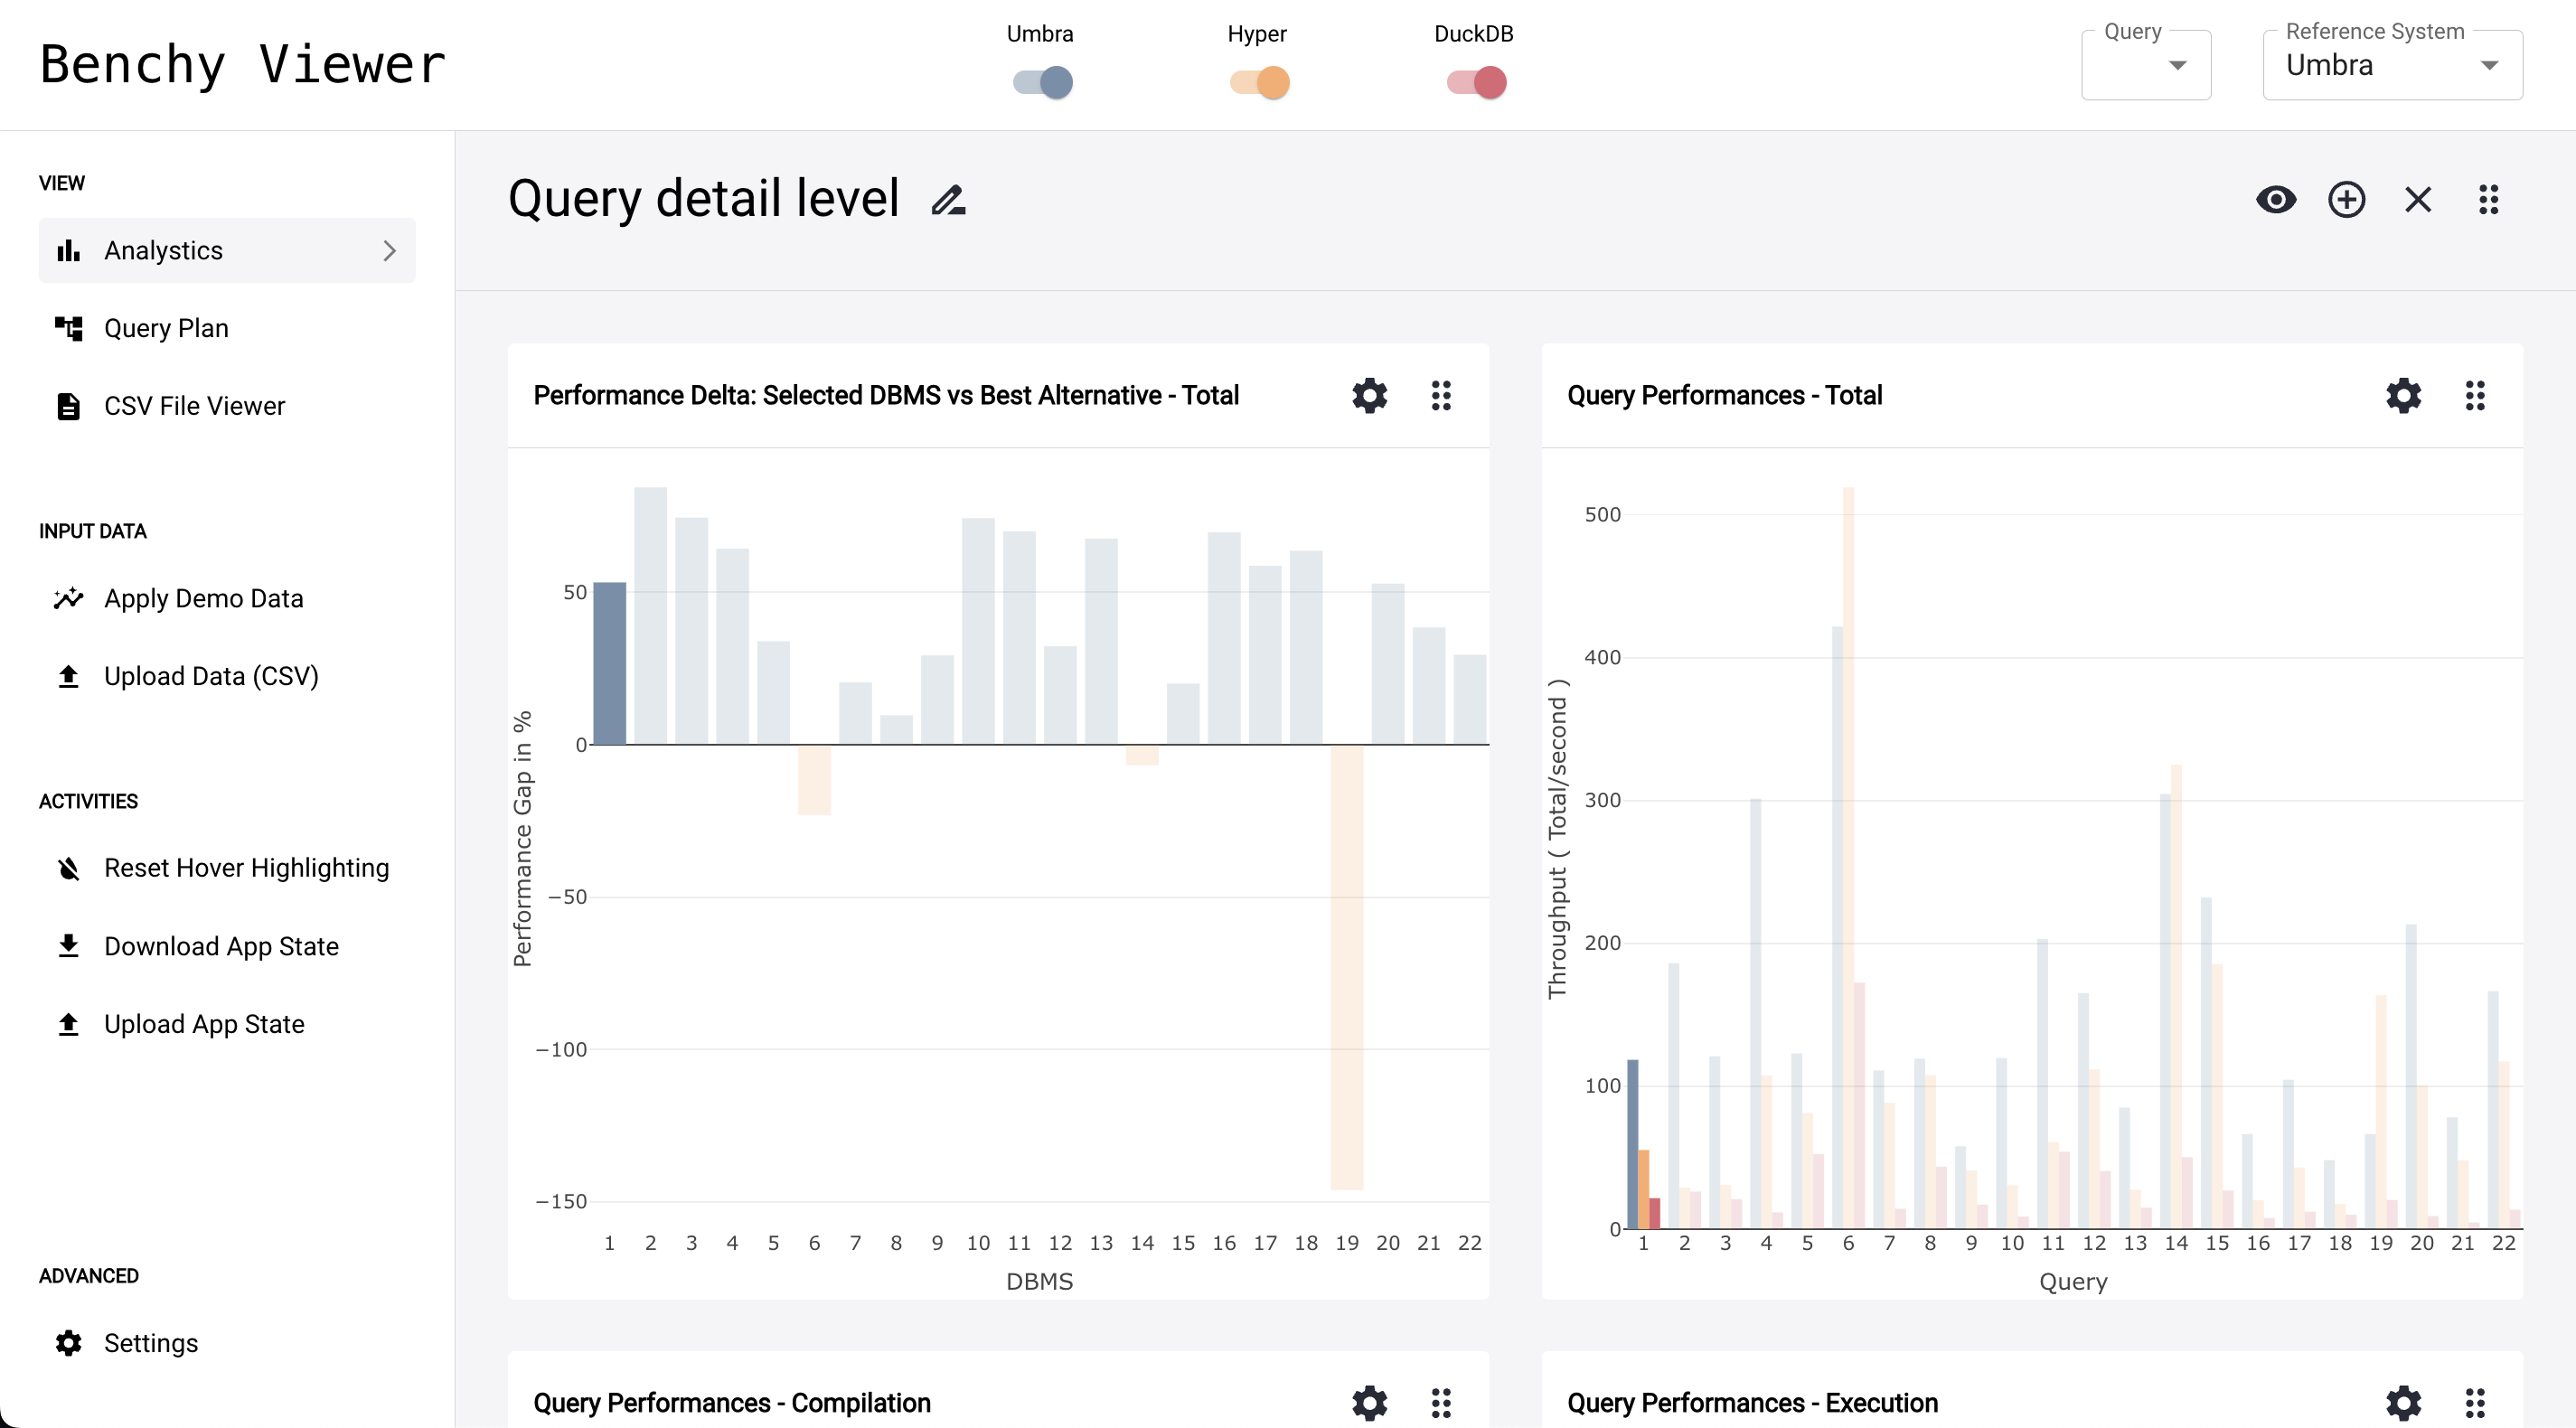
\includegraphics[width=\linewidth]{figures/app.png}
      \caption{Analytics Dashboard.}
        \label{fig:abstract-page}
    \end{subfigure}
    \hspace{0.5cm} % Adjust the horizontal space between the figures
    \begin{subfigure}[b]{0.3\linewidth}
      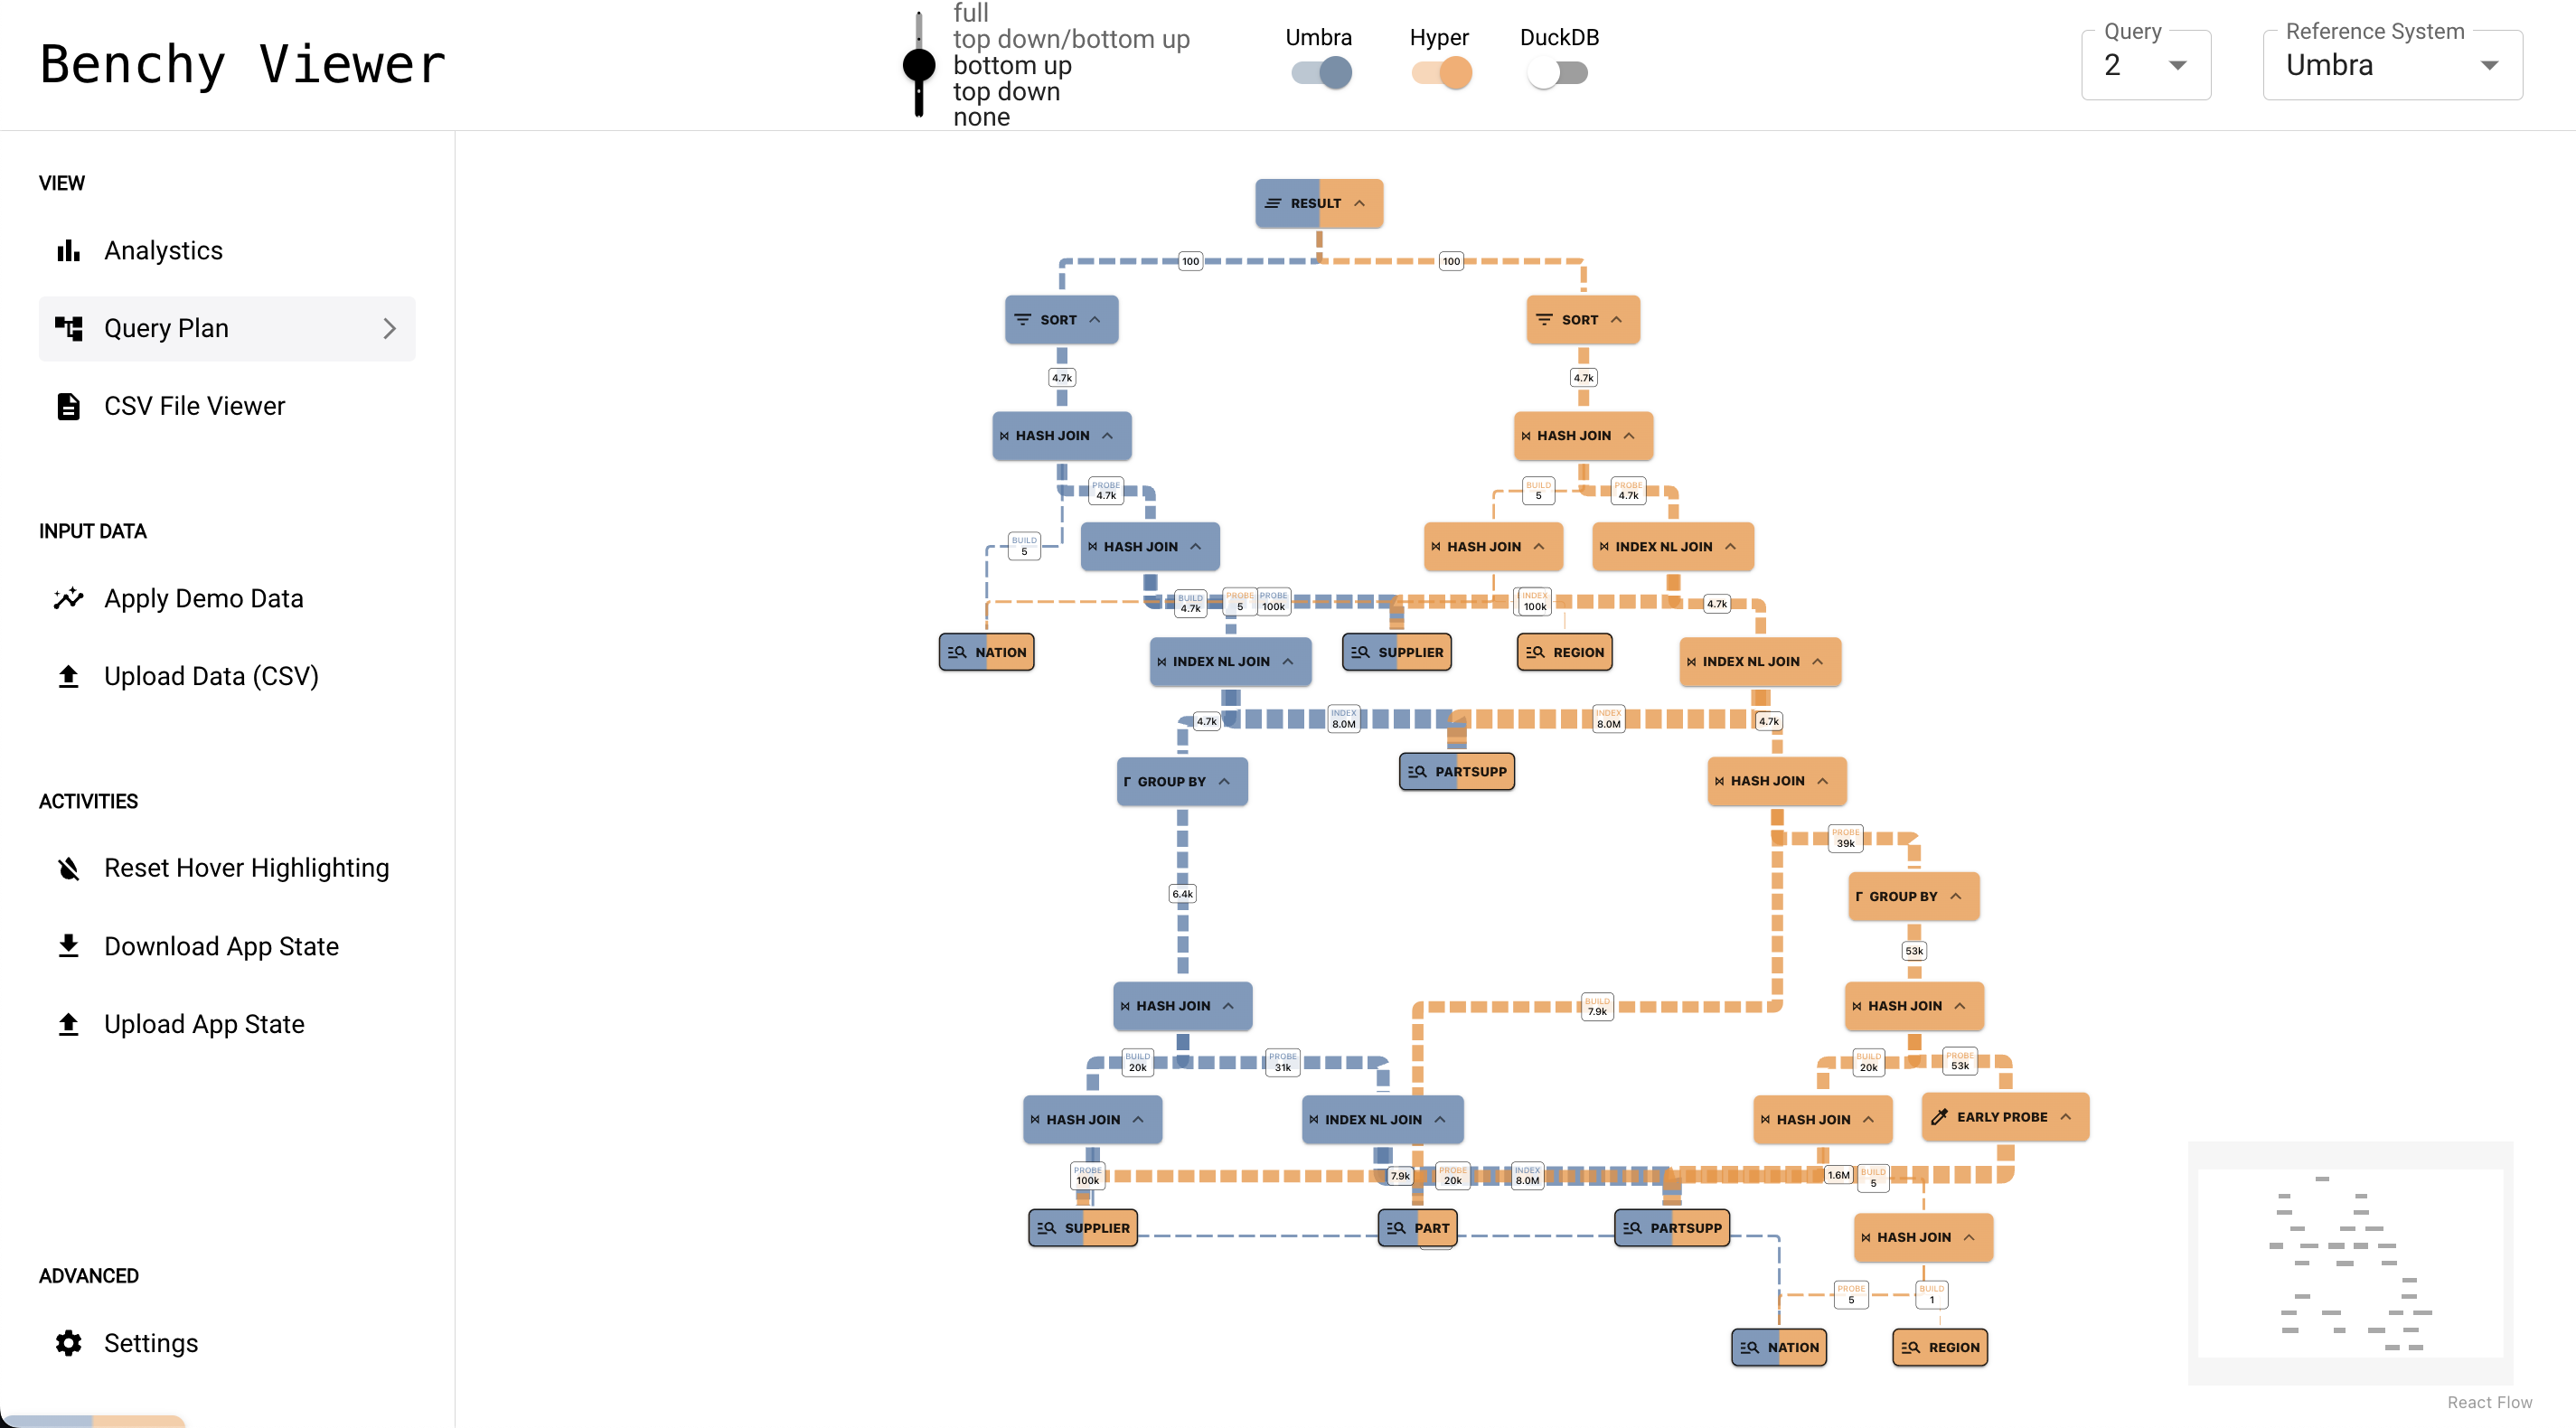
\includegraphics[width=\linewidth]{figures/app-query-plan.png}
      \caption{Query Plan View.}
        \label{fig:abstract-query-plan}
    \end{subfigure}
    \hspace{0.5cm} % Adjust the horizontal space between the figures
    \begin{subfigure}[b]{0.3\linewidth}
      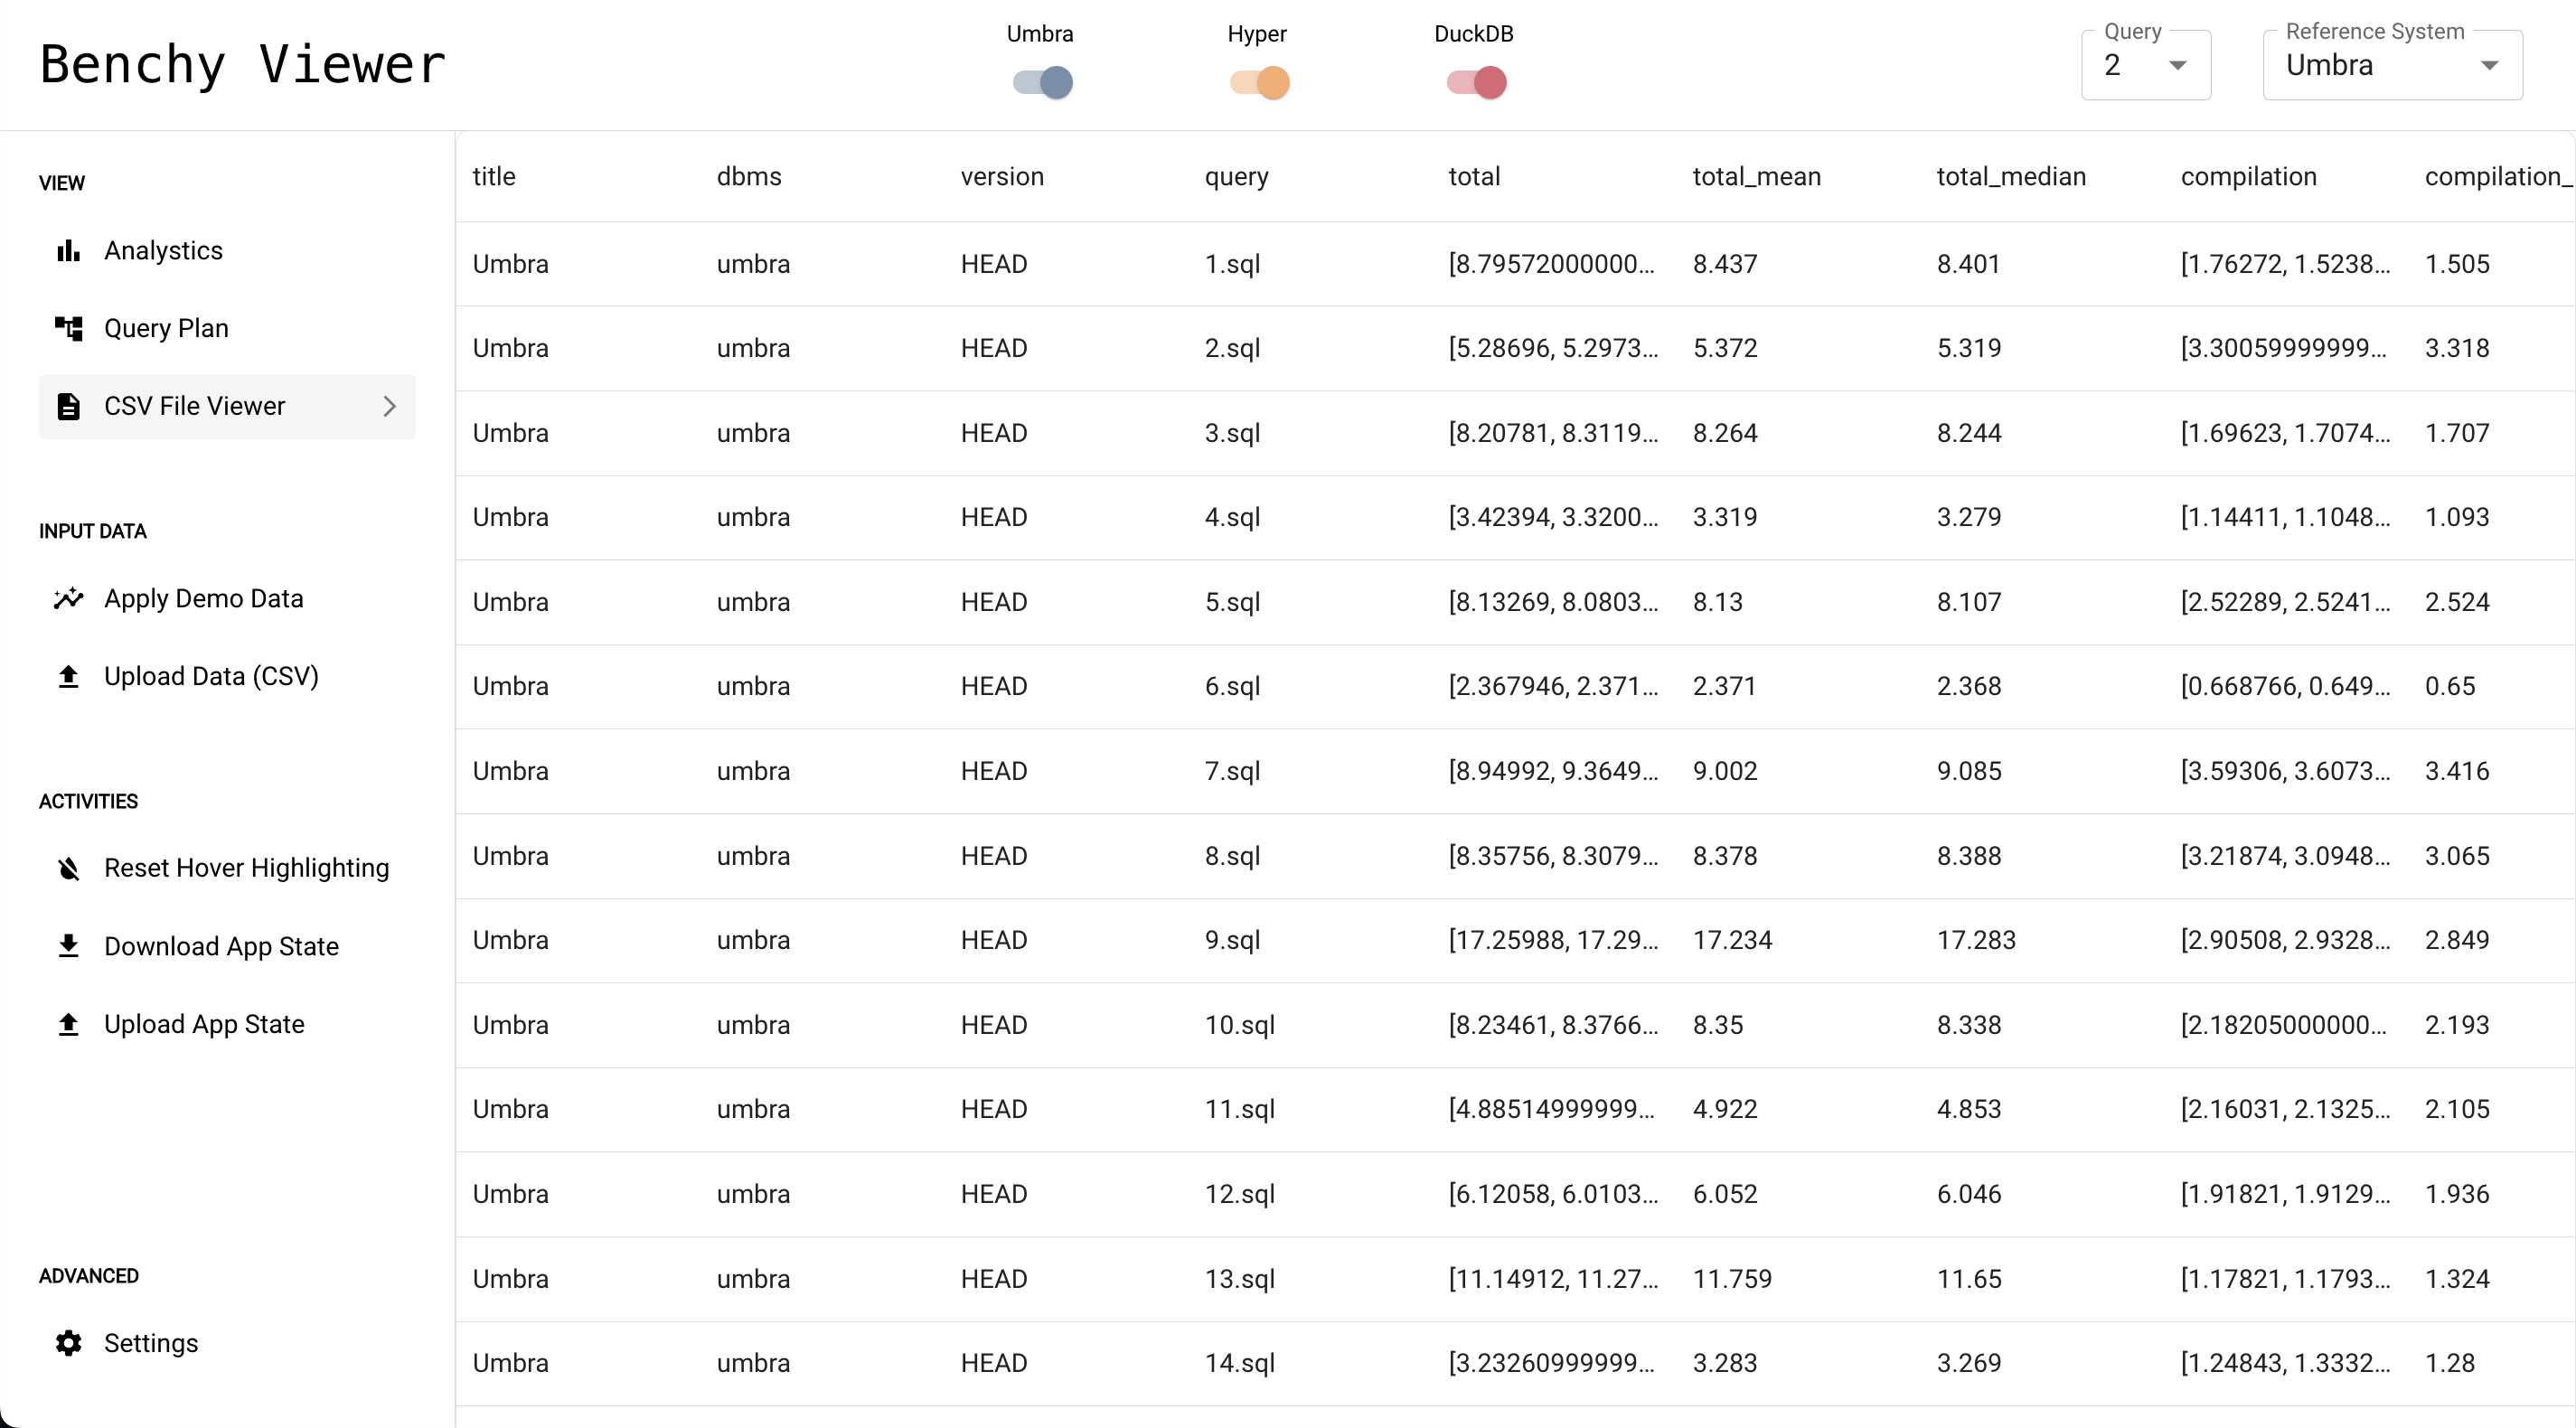
\includegraphics[width=\linewidth]{figures/app-data-viewer.png}
      \caption{Input File Viewer.}
        \label{fig:abstract-data-viewer}
    \end{subfigure}
    \caption{Benchy Viewer: Tool for analyzing performance measurements of database systems through interactive visualizations.}
    \label{fig:abstract}
  \end{figure}

%   In the ever-evolving landscape of database systems,

% This master thesis introduces the Benchy Viewer, a web-based serverless application designed for interactive exploration and analysis of performance data from various database systems. The primary objective is to empower database engineers by providing an intuitive platform for in-depth query execution analysis.\\
% We focus on consolidating a variety of interactive diagrams that portray diverse information content, aiming to elevate the interpretation of profiling data in database systems. The scope delineates the primary questions guiding the investigation, with a focus on the design and development of the Benchy Viewer application, as well as the exploration of statistical methods for analyzing performance data in database systems.


% The thesis structure navigates through related work, theoretical foundations, and the implementation of the Benchy Viewer. It scrutinizes the theoretical underpinnings of database systems, delves into datasets and data structures, and unveils the intricacies of implementation, emphasizing features, interaction capabilities, and design guidelines.

Embarking on the intricate journey of database performance optimization, this thesis underscores the pivotal role of performance analysis in benchmark data. A foundational understanding of system intricacies is paramount for overall performance enhancement. Recognizing the indispensability of visualizations in this analytical process, our work introduces the Benchy Viewer, a web-based serverless application meticulously designed to elevate the analysis of performance benchmark data.

Our main focus is on delivering interactive visualizations through an intuitive user interface, creating an environment where database developers can seamlessly navigate and interpret benchmark data. Developed using React, the Benchy Viewer stands out for its flexibility and the degree of interaction embedded in its intuitive user interface, empowering developers to dynamically explore benchmark data. It offers diverse perspectives, allowing users to view performance metrics from various angles, including a comparison perspective of query plans across different system instances, adding a layer of depth to performance analysis.

Built on an extensible architecture, the Benchy Viewer paves the way for future improvements. Its adaptability enables the incorporation of additional visualizations and analytical perspectives. 
In essence, the Benchy Viewer emerges as a transformative tool, achieving varied perspectives through interactive visualizations and an intuitive user interface, while its extensible architecture opens avenues for continuous enhancement.







\microtypesetup{protrusion=false}
\tableofcontents{}
\microtypesetup{protrusion=true}

\mainmatter{}

% !TeX root = ../main.tex
% Add the above to each chapter to make compiling the PDF easier in some editors.

\chapter{Introduction}\label{chapter:introduction}
Interactive performance visualization is a powerfull skill and plays a vital role for the demonstration of meaningful data insights in the context of performance measurements. Our goal is to use this powerfull skill properly to enable potential optimization possibilities for compiling database systems.

\section{Motivation}
\section{Technical Background}
\subsection{React}
\subsection{Redux}
\subsection{React Sweet State//}
\subsection{Plotly}
\subsection{React-Flow}
\subsection{Material UI}
\section{Existing Visualization of Performance Data of Umbra //PDF }
\section{Research objectives}
\section{Scope and contribution of the thesis}
\section{Thesis structure}


% TODO: add more chapters here 
% !TeX root = ../main.tex
% Add the above to each chapter to make compiling the PDF easier in some editors.

\chapter{Related Work}\label{chapter:relatedWork}
In this chapter, we give an overview about the existing work in the domain of the visualization of database performance profiling.
We will investigate the importance of optimizing query executions in database systems and the role of visualizations in identifying potential improvements.
As performant measurement and analysis play a crucial role in developing and optimizing database systems, 
it is essential to examine the state-of-the-art techniques and tools that have been used in this domain.
We will also cover a visualization tool closely associated with this thesis, as its key feature is integrated into the Benchy Viewer.

\section{Performance Visualization}
Sektion eher in Background
\textcolor{red}{Todo: Was es alles in dieser Domain gibt. Was effektiv ist und wir benutzen. Was wir nicht benutzen  mit Begründung.  }

\section{Database Performance Profiling }

Performance profiling in database systems is crucial for optimizing their execution regarding achieving optimal hardware utilization and query efficiency.
Profiling the performance of database systems involves collecting and analyzing various performance metrics during query execution.
\\Besides profilers presenting results at the instruction and function granularity, a paper on "Profiling Dataflow Systems on Multiple Abstraction Levels" \cite{profiling-dataflow} proposes a solution that tracks the code generation process and aggregates profiling data to higher abstraction levels. This approach helps bridging the semantic gap between low-level profiles and high-level constructs, making it easier for developers to interpret profiling results and identify bottlenecks and hotspots in the system. The paper introduces the concept of Tailored Profiling, which extends the compilation steps to annotate the generated code with metadata. This enables the mapping of profiling results back to desired abstraction levels and provides more understandable profiling data.
Building on the insights from this work, the opportunity arises to create more meaningful visualizations regarding the dataflow in system performance profiling.
\\ An essential concept of this thesis is to build upon the concepts of tailored profiling to gain a deeper understanding of the system's performance and support the location of potential optimization possibilities. Thus, we integrate an intuitive and interactive query plan visualization feature that is able to break down complex queries into their constituent operators and pipelines. We clarify further details about the query plan in section \ref{subsec:semantic-diff} and in chapter X (Implementation) \textcolor{red}{Todo: Chapter linking}.

\section{Related visualization tools}

This section explores related visualization tools that aid developers analyse their database system queries, with a specific focus on performance visualization. We will go through the Query Plan Difference Visualiser and the Umbra Profiler \textcolor{red}{Todo: Zitat}, which are both tools, that are strongly related to the Benchy Viewer. 


\subsection{Query Plan Difference Visualiser}
\label{subsec:semantic-diff}

The efficiency of a database system's query execution relies on the physical execution plan it generates.  Given the complexity of finding the best plan, the comparison of query plans both within a single system and accross different systems has garnered attention. This comparative analysis aims to gain valuable insights and identify potential optimisation opportunities. Previous efforts in this direction have mainly focused on quantitative metrics, in particular the total cost of the plan.
\begin{figure}[h]
    \centering
    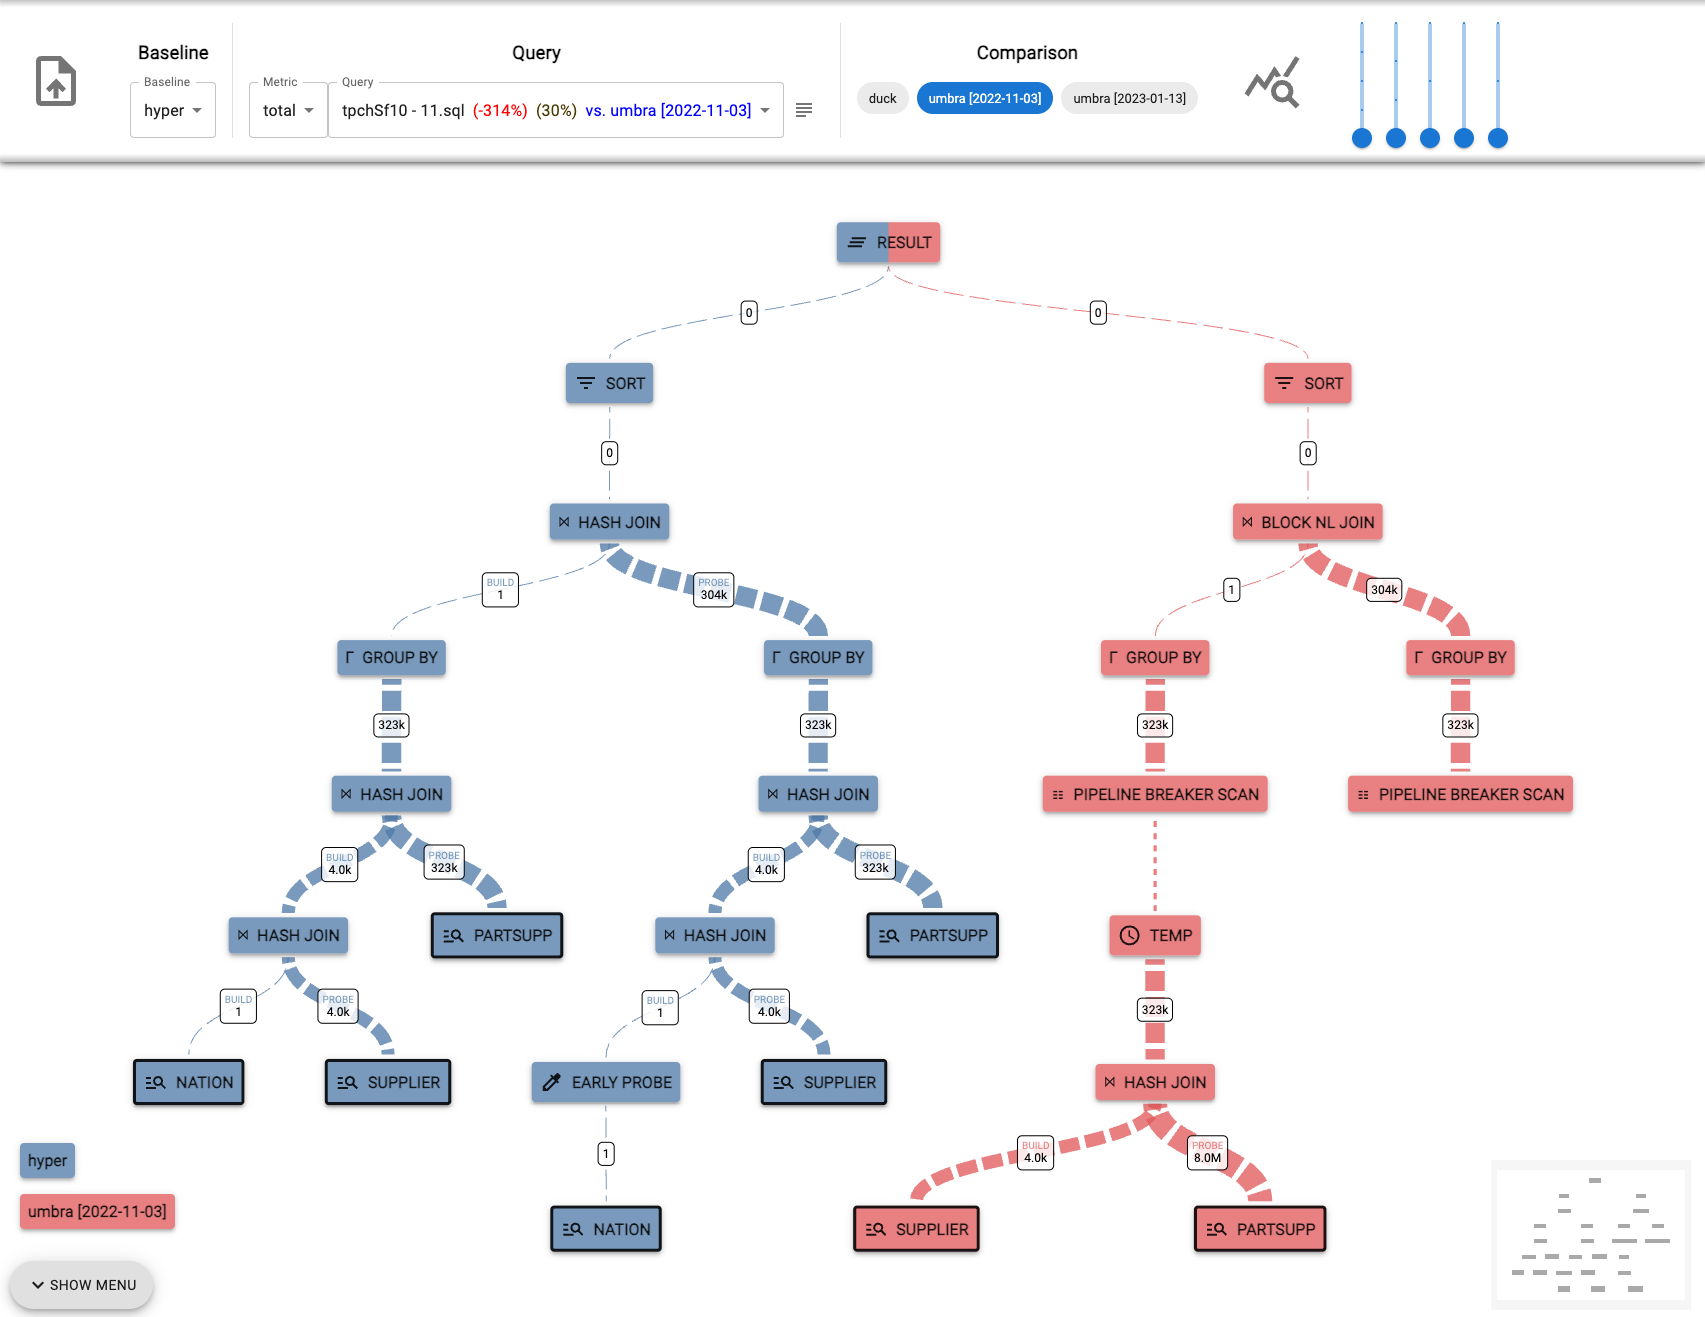
\includegraphics[width=0.8\linewidth]{figures/semantic-diff.png}
    \caption{Query Plan Difference Visualiser}
    \label{fig:semantic-diff}
  \end{figure}

\noindent 
Query execution plans describe the step-by-step hierarchical sequence of physical operations that a database system uses to process a particular SQL query. The fascinating aspect of this is that identical queries can result in different plans when processed by different database systems. This variability in plan generation can have a significant impact on overall performance.
\\The Query Plan Difference Visualiser is a web application that compares and visualises these physical query execution plans from different relational database systems, as shown in Figure~\ref{fig:semantic-diff}. It is designed for database developers who want to inspect the correlation between variations in query execution speed and the respective query plans. Through enhanced hierarchical differencing algorithms with semantic information about query plans, the tool is able to interactively capture and present  the difference between query plans. This is particularly useful for comparing different database systems or different versions of the same system when varying query plans are used by the systems under test to process the same query. Furthermore, it provides the flexibility to pick an arbitrary number of systems for which to compare plans and select a metric for evaluating query performance, such as total runtime or compilation time. For the given metric, it directly shows the difference between the baseline system and the better system.
\\ Once a query plan is initialized, the comparative tool provides the option to improve the clarity of the query plan visualization using various configuration settings. For instance, the tool offers a match mode selection, allowing users to capture the tree from, e.g., a top-down or bottom-up matching perspective. With the Expand and Collapse feature, users can collapse entire subtrees and selectively expand specific child nodes, customizing the focus of the visualization and tailoring the area of attention to the most interesting parts of the tree.
For query plans containing Directed Acyclic Graph (DAG) edges, such as the Pipeline Breaker Scan operator in Umbra, the tool offers support to include these DAG edges and consider them during the matching process. Additionally, to enable more effective comparisons against systems that generate non-DAG-shaped plans, an option is available to replicate subtrees instead.
\\ Database developers often find value in comparing query plans, particularly when they have thoroughly examined different results using quantitative metrics. 
Therefore, we decided to integrate the Query Plan Difference Visualiser with its core features of comparing query plans. In addition to visualising quantitative metrics from different database systems within the Benchy Viewer, the incorporation of the Query Plan Difference Visualiser with its capabillities will further enhance our objective of simplifying the detection of performance bottlenecks in query execution and optimizing database systems.

Hence, the Query Plan Difference Visualiser is strongly related to this thesis and we will dive deeper into the integration of the comparative tool in Chapter X. \textcolor{red}{Todo: Chapter linking}



\subsection{Umbra Profiler}
The Umbra Profiler is a tool that enables in-depth analysis for identifying bottlenecks in query execution processes of the database system Umbra.
\\ It is integrated with a backend application for preparing extensive profiling data and offers multiple perspectives, including a runtime dashboard, a memory dashboard, and an instruction dashboard, each depicting distinct information, as illustrated in Figure~\ref{fig:umbra-profiler}.

\begin{figure}[h]
  \centering
  
\includegraphics[width=1\linewidth]{figures/umbra-profiler.png}
  \caption{Umbra-Profiler: A tool for analyzing and profiling Umbra’s compiling queries. From left-to-right: runtime dashboard, memory dashboard, and instruction dashboard.}
  \label{fig:umbra-profiler}
\end{figure}

\noindent 
The runtime dashboard is the default view that appears after providing recorded hardware samples of a query execution. It offers an initial overview of the query execution structure, allowing users to analyze the activity of specific processor events, operators, and pipelines over time. Abnormalities in execution, such as resource-intensive operations, can be identified, aided by visualizations including key performance indicators, activity histograms, bar charts, query plans, sunburst charts, and swim lanes.
\\The memory behavior dashboard focuses on memory access patterns in query execution. It offers memory heatmaps for each operator, showing either absolute memory accesses or sequential memory address differences.
\\The instruction Dashboard facilitates detailed analysis of query execution using Umbra Intermediate Representation (UIR) \textcolor{red}{Zitat} instructions. It allows comparison of UIR instructions with query plans to identify performance problems based on costs and occurrences. 
\\Similar to the Benchy Viewer, the goal is to support database engineers in optimizing query execution by providing an interactive user interface, enabling an effective in-depth analysis process. 
\\The Umbra Profiler is designed based on the innovative Tailored Profiling approach \cite{profiling-dataflow}, where the connection between query plans and compiled code is maintained. This technique was previously unaddressed by standard profilers and is now used in both the Umbra Profiler and the Benchy Viewer.  
\\However, unlike the Benchy Viewer, the Umbra Profiler is focused to operate exclusively with the database system Umbra. In contrast, the Benchy Viewer has the versatility to function with multiple database systems or multiple instances of a single database system.
\\In broad terms, the Umbra Profiler is primarily designed for in-depth analysis of query performance within a single database system, while the Benchy Viewer is oriented towards its comparative function, enabling the comparison of queries executed by different instances. This comparative approach is the main essence  of the concept of the Benchy Viewer, which aims to enhance the understanding of differences between database instances.

An effective scenario that synergizes the Benchy Viewer and the Umbra Profiler would involve identifying intriguing queries using the Benchy Viewer and subsequently conducting comprehensive analyses using the Umbra Profiler.



% !TeX root = ../main.tex
% Add the above to each chapter to make compiling the PDF easier in some editors.

\chapter{Theoretical Foundations}\label{chapter:theoreticalFoundacions}

In this chapter, we investigate the theoretical foundations by examining database performance measurements and in the next step describing used datasets and the data structure.\\We will start by discussing the characterisitcs of database systems and elaborate on the significance of performance measurements in this context. Additionally, we will outline the common performance metrics, that play a central role in the evaluation of performance analysis.
\\ For clarifying used datasets and the data structure, we commence by describing the utilized performance data, followed by giving an overview of the structure of the Benchy Viewer's input file containing the performance measurements. Moreover, the data prepration for this input file will be explained.

\section{Database Systems and Performance Measurements}
Performance measurement and analysis are fundamental in the realm of database systems. They offer valuable insights into system behavior, helping to pinpoint bottlenecks and optimization opportunities. This process is crucial not only for evaluating one's own system but also for making meaningful comparisons with other systems. Visualisations play a pivotal role in understanding performance data and are often used to convey complex findings effectively.
To interpret performance data effectively, we begin by understanding the characteristics and core traits of a Database System.

\subsection{Characteristics of Database Systems}
Database systems are complex structures that manage and store vast amounts of data efficiently, involving interrelated factors that must be finely tuned to ensure optimal performance.\\
One of the fundamental functions of a database system is query processing. A query is essentially a request for specific information from the database. This involves receiving and then executing that query. The process includes tasks like parsing, optimization, and execution.\\
Queries go through two main phases: compilation and execution. \textcolor{red}{Figure mit Compilation und Execution} During compilation, the query is transformed into an execution plan. This plan outlines the steps the system should take to retrieve the requested data. In the execution phase, the system follows this plan to fetch the data.\\
Query plans are roadmaps that guide how a database executes queries, with operators as specialized components responsible for specific actions. Operators, like selection and join operators, perform data operations during query execution, such as filtering and combining data. Optimizing query plans is vital for database efficiency, with query optimizers selecting the best plan considering factors like data distribution and hardware capabilities.\\
Query processing can be time-consuming due to various challenges. For instance, complex queries, large datasets, and suboptimal query plans can lead to slow performance. Identifying and overcoming these challenges is essential for improving system efficiency.

Understanding these characteristics is key to understanding the complexity of database performance. Challenges such as optimising query plans and dealing with large data sets are common, and manual assessment is often impractical.\\
The need for objective metrics is therefore obvious, making performance measurements essential for targeted optimisations. Due to the complexity of these metrics, visualisation techniques are invaluable for easier interpretation and analysis.\\
In the next section, we will explore the important role of performance measurements and their visualisation in improving database efficiency.


\subsection{Importance of Performance Measurements}
Database systems are the core of a wide range of applications. Consequently, their performance matters not just in terms of user-friendliness and reliability, but also in terms of efficiency. Performance measurements play a central role in this context.\\
One of the key advantages of performance measurements lies in their capacity to assist in optimization efforts. By quantifying performance in a series of metrics, database developers can pinpoint precisely where bottlenecks occur, whether it is in the compilation phase, the query plan, data retrieval, or any other component of the database system. This focused approach minimizes the trial and error often involved in performance tuning and directs resources toward the most impactful modifications.\\
Furthermore, bottlenecks and areas with room for improvement are often not obvious. With the aid of performance measurements, these elements come into sharp focus. Measurements can reveal, for example, if the system's weak point lies in query compilation or if the query plan needs to be optimized. Understanding and interpreting the findings correctly is crucial for making informed decisions on where to prioritize improvement efforts.\\
Another fundamental aspect is scalability. In a world where data is continuously growing, the scalability of a database system becomes a certain priority, because data volumes continue to grow. Performance measurements can identify the limitations of a system as it scales, revealing performance degradation points before they become critical bottlenecks. This approach is not only applied to solve current needs of data volume, but is also contributing to the system's scalability for the future.\\
Referring back to the introduction's implication, the complexity of performance metrics can often be overwhelming. Visualisation techniques become invaluable tools in this context. By translating numerical data into graphical elements, these visualisations can illuminate patterns and trends that could otherwise be easily overlooked, offering an intuitive and interactive way to understand the performance bottlenecks and operational nuances.

In summary, performance measurements are essential in the effective management and optimization of complex database systems. With these basic principles in mind, the next section examines common performance metrics for evaluating database systems, which serve as the quantitative backbone for the analyses and visualisations discussed here.

\subsection{Common Performance Metrics}
Understanding the importance of performance measurements in database systems necessitates a deeper dive into the specific metrics that help analyse various aspects of performance. This section explores effective metrics and how they are used within this domain, which indicates the desired functionalities of the Benchy Viewer in terms of interaction and visualisation.\\
In the paper "Bringing Compiling Databases to RISC Architectures" \cite{Bringin-Compiling-Databases-to-RISC} the compilation performance of the dominant x86-64 server architecture is contrasted  with the new introduced code generator designed for AArch64-based systems. This is interesting for the Benchy Viewer as it conducts a comparative analysis of different perspectives in terms of performance,  leveraging specific performance metrics that are also visually represented.\\ 
The paper utilizes both quantitative and subjective performance metrics when addressing the query compilation strategy. However, for the scope of our visualisation, we focus on the quantitative metrics. Relying on quantitative metrics allows for clear, objective visualisation that can represent performance differences, whereas subjective metrics does not offer the same level of clarity and consistency in a visual representation.\\
Here one of the most central metrics is the throughput, a key metric in databases, measures the number of processed tuples per second and is a primary optimization target. In the context of compiling databases, throughput is primarily influenced by the quality of the generated machine code for queries.\\
Another fundamental metric is the latency, which is the time needed for generating and compiling query code before execution, with lower latency being particularly important for real-time transactional systems.\\
With these two metrics, the paper shows an intuitive and clear overview of how different database instances perform on the TPC-H benchmark, as demonstrated in Figure~\ref{fig:risc-metrics}.

\begin{figure}[h]
  \centering
  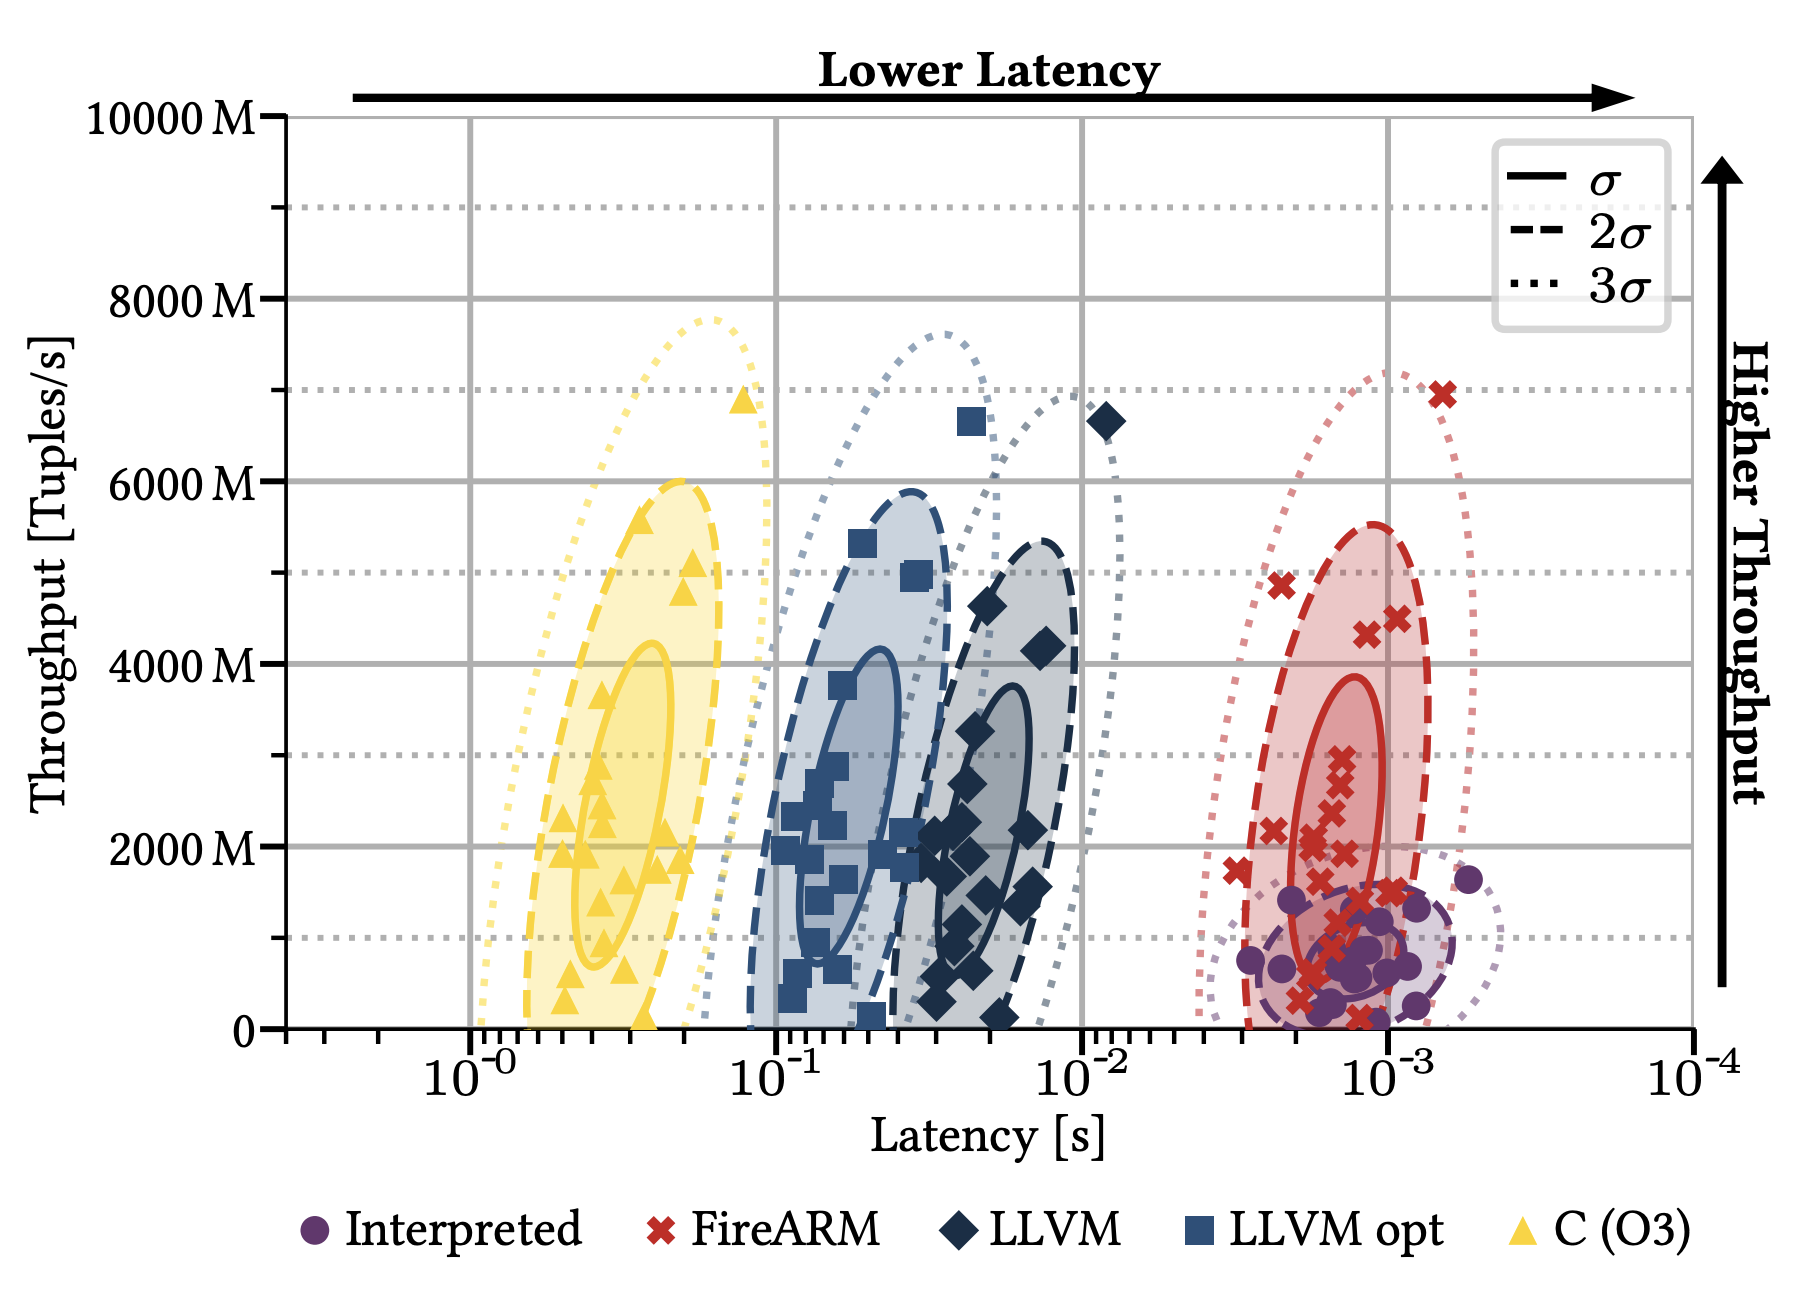
\includegraphics[width=0.8\linewidth]{figures/risc-metrcis-visualization.png}
  \caption{Visualisation example of compile-time and throughput of different query-compilation strategies running the TPC-H benchmark \cite{Bringin-Compiling-Databases-to-RISC}.}
  \label{fig:risc-metrics}
\end{figure}

\noindent

The visualisation presents a scatter plot that groups query results into clusters, with each cluster representing a database instance by a distinct color. The Y-axis displays the throughput in tuples per second, while the X-axis shows the latency in seconds, which is a descending value from left to right. Additionally, arrowed labels point to the preferred values: higher values on the Y-axis and lower on the X-axis. Thus, top-right-corner values represent optimal performance, allowing viewers to quickly identify well-performing database instances as well as the performance differences between instances.\\
In this illustration, the system highlighted in red is notable for its low latency and high throughput. Conversely, the system marked in yellow has the poorest latency performance. The instance in purple also stands out, boasting the lowest latency, but it lags behind in terms of throughput.

In the context of performance metrics, the Benchy Viewer should be capable of visualizing the key differences between instances in an intuitive and effective way. 

Besides grouping the query results into clusters, with each cluster representing a database instance, it would also be beneficial to have the flexibility to choose a specific metric for this categorization. For instance, if a database developer is primarily concerned with the metrics of execution time and throughput, they should have the option to shape the data visualisation based on these metrics.

Up next, we'll explore the dataset that is consumed by the Benchy Viewer to offer all the data and performance metrics within the analytical visualisations. We'll detail the data structure and how the data is prepared to get in this shape.

\section{Used Datasets and Data Structure}
\subsection{Description of the Utilized Performance Data}
\subsection{Structure of the CSV File with Performance Measurements}
\subsection{Data Preparation}



% !TeX root = ../main.tex
% Add the above to each chapter to make compiling the PDF easier in some editors.

\chapter{Example}\label{chapter:example}

\section{Section}
Citation test~\parencite{latex}.

Acronyms must be added in \texttt{main.tex} and are referenced using macros. The first occurrence is automatically replaced with the long version of the acronym, while all subsequent usages use the abbreviation.

E.g. \texttt{\textbackslash ac\{TUM\}, \textbackslash ac\{TUM\}} $\Rightarrow$ \ac{TUM}, \ac{TUM}

For more details, see the documentation of the \texttt{acronym} package\footnote{\url{https://ctan.org/pkg/acronym}}.
\subsection{Subsection}

See~\autoref{tab:sample}, \autoref{fig:sample-drawing}, \autoref{fig:sample-plot}, \autoref{fig:sample-listing}.

\begin{table}[htpb]
  \caption[Example table]{An example for a simple table.}\label{tab:sample}
  \centering
  \begin{tabular}{l l l l}
    \toprule
      A & B & C & D \\
    \midrule
      1 & 2 & 1 & 2 \\
      2 & 3 & 2 & 3 \\
    \bottomrule
  \end{tabular}
\end{table}

\begin{figure}[htpb]
  \centering
  % This should probably go into a file in figures/
  \begin{tikzpicture}[node distance=3cm]
    \node (R0) {$R_1$};
    \node (R1) [right of=R0] {$R_2$};
    \node (R2) [below of=R1] {$R_4$};
    \node (R3) [below of=R0] {$R_3$};
    \node (R4) [right of=R1] {$R_5$};

    \path[every node]
      (R0) edge (R1)
      (R0) edge (R3)
      (R3) edge (R2)
      (R2) edge (R1)
      (R1) edge (R4);
  \end{tikzpicture}
  \caption[Example drawing]{An example for a simple drawing.}\label{fig:sample-drawing}
\end{figure}

\begin{figure}[htpb]
  \centering

  \pgfplotstableset{col sep=&, row sep=\\}
  % This should probably go into a file in data/
  \pgfplotstableread{
    a & b    \\
    1 & 1000 \\
    2 & 1500 \\
    3 & 1600 \\
  }\exampleA
  \pgfplotstableread{
    a & b    \\
    1 & 1200 \\
    2 & 800 \\
    3 & 1400 \\
  }\exampleB
  % This should probably go into a file in figures/
  \begin{tikzpicture}
    \begin{axis}[
        ymin=0,
        legend style={legend pos=south east},
        grid,
        thick,
        ylabel=Y,
        xlabel=X
      ]
      \addplot table[x=a, y=b]{\exampleA};
      \addlegendentry{Example A};
      \addplot table[x=a, y=b]{\exampleB};
      \addlegendentry{Example B};
    \end{axis}
  \end{tikzpicture}
  \caption[Example plot]{An example for a simple plot.}\label{fig:sample-plot}
\end{figure}

\begin{figure}[htpb]
  \centering
  \begin{tabular}{c}
  \begin{lstlisting}[language=SQL]
    SELECT * FROM tbl WHERE tbl.str = "str"
  \end{lstlisting}
  \end{tabular}
  \caption[Example listing]{An example for a source code listing.}\label{fig:sample-listing}
\end{figure}


\appendix{}

\microtypesetup{protrusion=false}

\addchap{Abbreviations}
\begin{acronym}
	\itemsep-.25\baselineskip
	\acro{TUM}[TUM]{Technical University of Munich}
	% TODO: add acronyms
\end{acronym}

\listoffigures{}
\listoftables{}
\microtypesetup{protrusion=true}
\printbibliography{}

\end{document}
